% Created by tikzDevice version 0.8.1 on 2015-11-15 21:50:56
% !TEX encoding = UTF-8 Unicode
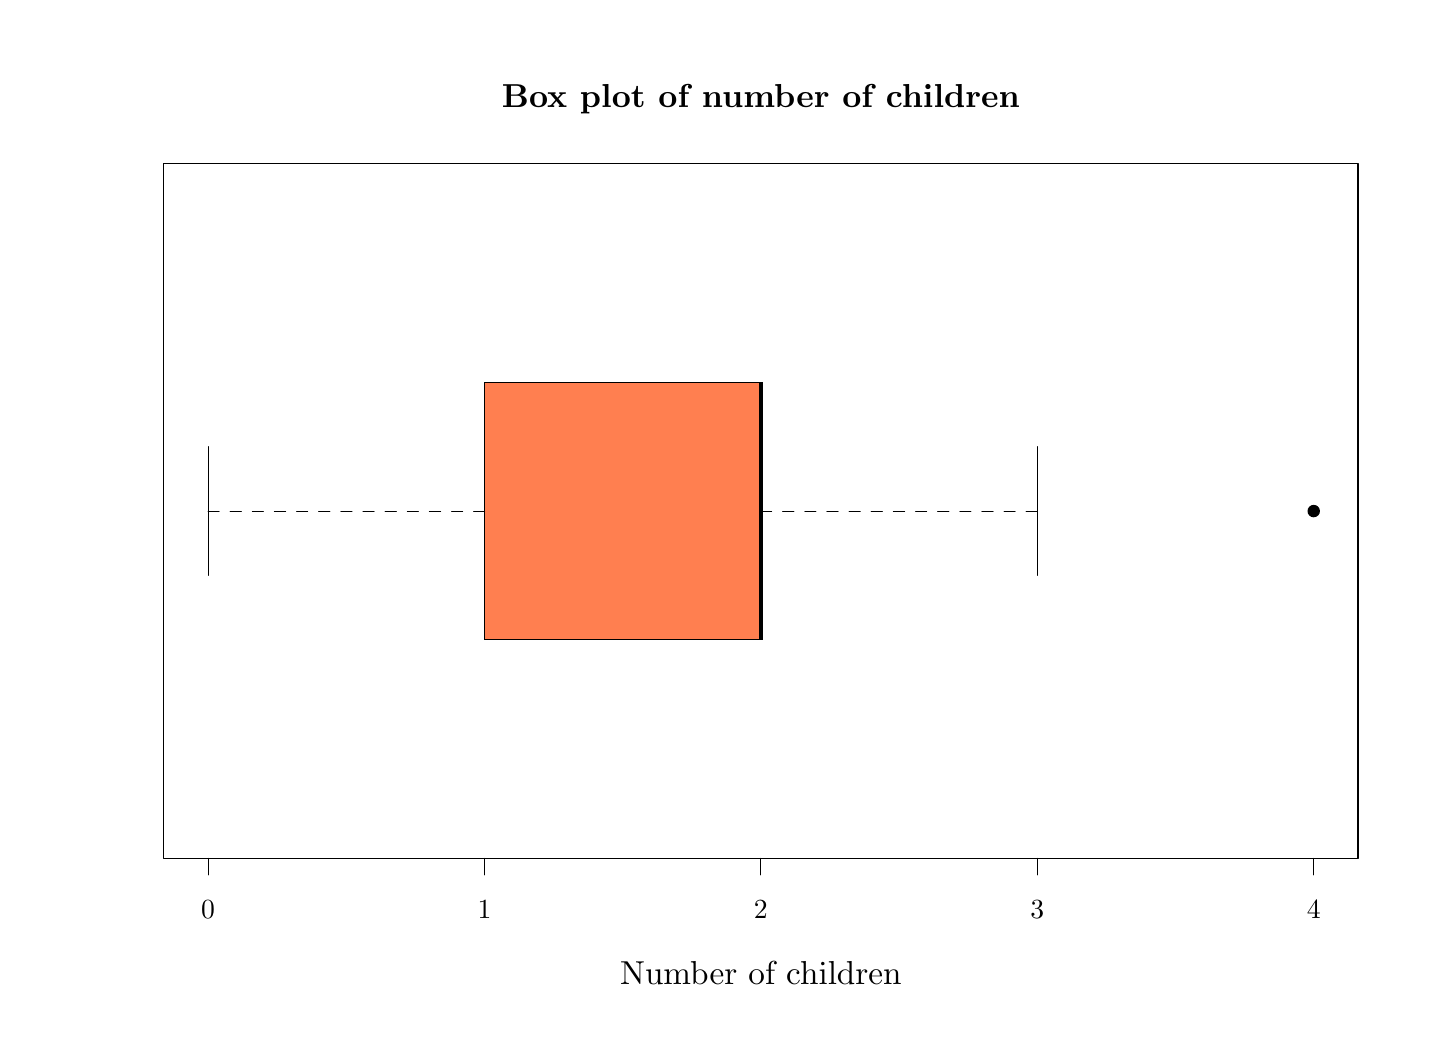
\begin{tikzpicture}[x=1pt,y=1pt]
\definecolor{fillColor}{RGB}{255,255,255}
\path[use as bounding box,fill=fillColor,fill opacity=0.00] (0,0) rectangle (505.89,361.35);
\path[draw,line width= 0.4pt,line join=round,line cap=round] ( 49.20, 61.20) --  (480.69, 61.20) --(480.69,312.15) -- (
49.20,312.15) -- ( 49.20, 61.20); 
\node[anchor=base,inner sep=0pt, outer sep=0pt, scale=  1.20] at (264.94,332.61) {\bfseries Box plot of number of children};
\node[anchor=base,inner sep=0pt, outer sep=0pt, scale=  1.20] at (264.94, 15.60) {Number of children};
\path[draw,line width= 0.4pt,line join=round,line cap=round] ( 65.18, 61.20) -- (464.71, 61.20);
\path[draw,line width= 0.4pt,line join=round,line cap=round] ( 65.18, 61.20) -- ( 65.18, 55.20);
\path[draw,line width= 0.4pt,line join=round,line cap=round] (165.06, 61.20) -- (165.06, 55.20);
\path[draw,line width= 0.4pt,line join=round,line cap=round] (264.94, 61.20) -- (264.94, 55.20);
\path[draw,line width= 0.4pt,line join=round,line cap=round] (364.83, 61.20) -- (364.83, 55.20);
\path[draw,line width= 0.4pt,line join=round,line cap=round] (464.71, 61.20) -- (464.71, 55.20);
\node[anchor=base,inner sep=0pt, outer sep=0pt, scale=  1.00] at ( 65.18, 39.60) {0};
\node[anchor=base,inner sep=0pt, outer sep=0pt, scale=  1.00] at (165.06, 39.60) {1};
\node[anchor=base,inner sep=0pt, outer sep=0pt, scale=  1.00] at (264.94, 39.60) {2};
\node[anchor=base,inner sep=0pt, outer sep=0pt, scale=  1.00] at (364.83, 39.60) {3};
\node[anchor=base,inner sep=0pt, outer sep=0pt, scale=  1.00] at (464.71, 39.60) {4};
\begin{scope}
\path[clip] ( 49.20, 61.20) rectangle (480.69,312.15);
\pause
\definecolor{fillColor}{RGB}{255,127,80}
\path[draw] (165.06,140.20) -- (165.06,233.15);
\pause
\path[draw] (264.94,233.15) --	(264.94,140.20);
\pause
\path[draw, fill=fillColor] (165.06,140.20) -- (165.06,233.15) --	(264.94,233.15) --	(264.94,140.20) --	cycle;
\path[draw,line width= 1.2pt,line join=round] (264.94,140.20) -- (264.94,233.15);
\pause
\pause
\path[draw,line width= 0.4pt,line join=round,line cap=round] ( 65.18,163.44) -- ( 65.18,209.91);
\path[draw,line width= 0.4pt,dash pattern=on 4pt off 4pt ,line join=round,line cap=round] ( 65.18,186.67) -- (165.06,186.67);
\pause
\path[draw,line width= 0.4pt,dash pattern=on 4pt off 4pt ,line join=round,line cap=round] (364.83,186.67) -- (264.94,186.67);
\path[draw,line width= 0.4pt,line join=round,line cap=round] (364.83,163.44) -- (364.83,209.91);
\pause
\path[fill] (464.71,186.67) circle (  2.25);
\end{scope}
\pause
\end{tikzpicture}
